\documentclass{article}
% This text is inserted in the beginning of all
% LaTex and Tex files I create.
%
% File created: Thu Apr  1 2010
% File name:    paper.tex
% Path:         /home/mroughan/Reports/Networking/Topology/Waxman/
%
% Matthew Roughan
% matthew.roughan@adelaide.edu.au
%
\usepackage{fancyhdr}
\usepackage{epsf}
\usepackage{subfig}
\usepackage{latexsym}
\usepackage{dsfont}
\usepackage{url}
\usepackage{times}
\usepackage{graphicx}
\usepackage{amsfonts}
\usepackage{amsmath}
\usepackage{ifthen}
\usepackage{verbatim}

\setlength{\headheight}{10mm}
\setlength{\headsep}{10mm}
\setlength{\topmargin}{0cm}
\setlength{\textwidth}{175mm}
\setlength{\textheight}{225mm}
\setlength{\oddsidemargin}{-10mm}
\lefthyphenmin=2
\righthyphenmin=3

\renewcommand{\baselinestretch}{1.0}
\renewcommand{\textfraction}{0.1}


\def\RR{\mathds{R}}
\def\CC{\mathds{C}}

\newcommand{\titlestr}{Known Results for the Line Picking Problem}
\rhead[]{{\small \titlestr}}
\lhead[{\small }]{}
\cfoot{}
\rfoot[]{{\rm\thepage}}
\lfoot[{\rm\thepage}]{}
\renewcommand{\footrulewidth}{0.4pt}
\pagestyle{fancy}

\newtheorem{theorem}{Theorem}[section]
\newtheorem{lemma}{Lemma}[theorem]
\newtheorem{corollary}[theorem]{Corollary}
\newtheorem{Def}{Definition}[section]


\begin{document}
\title{\titlestr}
\author{Matthew Roughan \;\;\; Eric Parsonage \;\;\; Jonathon Tuke \\
 School of Mathematical Sciences \\
 University of Adelaide \\
 \url{ <{matthew.roughan,eric.parsonage,}@adelaide.edu.au> } }
\maketitle

\begin{abstract}

\end{abstract}

\section{Introduction}

The {\em line picking} problem is a standard problem in stochastic
geometry, where we pick lines at random from some region. The typical
questions one asks are what will then mean line length be? What will
the Probability Density Function (PDF) be?

This brief note describes the current list of known PDFs, and where
they were derived, as well as the current set of code to calculate
these. 

The code is written in C with minimal external dependencies, and with
suitable wrapper functions for Matlab and R, to allow it to be run on
a wide variety of systems.


\section{Problem Definition}

formalities

  -- 2 points, uniformly chosen at random (though there are
  generalizations)


\section{Known Results}
\label{sec:known}


The Waxman graph has been analysed in some detail, starting first with
analysis of points chosen randomly in the plane. Such points form a
spatial Poisson process across the region of interest. Much analysis
has considered such processes, and we will only repeat directly
relevant results here. The most recondite result concerns the
distribution of distances between two points chosen randomly in the
unit square.  The probability density function of distances between
two (uniformly) randomly chosen points on the unit square is given in
\cite{weisstein:_squar_line_picking}, as
\begin{equation}
  \label{eq:square_line}
  g(t) = \left\{ \begin{array}{ll}
      2t (t^2-4t+\pi), & \mbox{ for } 0 \leq t \leq 1, \\
      2t \left[4 \sqrt{t^2-1} - (t^2+2-\pi) - 4 \tan^{-1} \left(\sqrt{t^2-1} \right)\right], 
               & \mbox{ for } 1 \leq t \leq \sqrt{2} . \\ 
    \end{array} \right.
\end{equation}
% http://mathworld.wolfram.com/SquareLinePicking.html
This is a rather complicated expression, but is easily evaluated
numerically. Alternatively, in
\cite{m.naldi05:_connec_of_waxman_graph} this expression was
approximated with a $\beta$ function, though given the requirements to
numerically evaluate that function there hardly seems any advantage.
Figure~\ref{fig:LinePicking} shows the shape of this distribution.
It is noteworthy that the distance distribution between two points
will also give the distribution of the distances of links in an
Erd\H{o}s-R\'enyi random graph constructed on a set of random points
on the square.

% In high dimensions, the points are spread ``more thinnly'' in the
% sense that their density on $n$-dimensional volumes will be lower, and
% hence, the distances between points will be larger. As a result,
% Waxman graphs in higher dimensions may become more sparse.

The general problem of choosing a line from some space has been called
a {\em line picking} problem, with many examples having been studied.

Numerically it is straight-forward to calculate the function $g(t)$
and its Laplace transform where the nodes are placed on irregular
regions of the plane. It simply requires computation of a double
integral. Note however, that even if we constrain nodes to lie in the
region, if the region is non-convex the links may cross the boundaries
of the regions. A simple example is the Waxman graph on a circular disc
of radius $R$. It has the advantage of isometry, or rotational
symmetry.  When we restrict the vertices (and edges) to a circle the
problem is still relatively easy to solve. The distance distribution
between random points in the a circle radius $R$ is given by
\cite{tu00:_circle_line} as
\begin{equation}
   g_R(t)= \frac{4t}{\pi R^2} \cos^{-1}\left( \frac{t}{2R} \right)
          - \frac{2t^2}{\pi R^3} \sqrt{ 1- \frac{t^2}{4 R^2} }. 
  \label{eqn:circle}
\end{equation}
This function is also shown (for $R=0.5$) in
Figure~\ref{fig:LinePicking} for comparison with the function on the
unit square. Interesting, despite noticable differences in these
functions, we found little difference between the critical ration
$-G'(s)/G(s)$ for large $s$ (small $\alpha$) suggesting the in these
cases the exact form of the region may be fairly unimportant.

Note that the asymptotic expansion of $\cos^{-1}(x) = \frac{\pi}{2} -
O(x)$, so the small $t$ expansion of $g_R(t) = 2 t/R^2$, which is
identical per unit area to the small $\alpha$ approximation for the square.

Another example, an approximation of which appears in
\cite{m.naldi05:_connec_of_waxman_graph} is the rectangle. The precise
form of the distance density for this case is given in \cite[Theorem
2.4.4]{mathai_geom} as
\begin{equation}
  g_{a,b}(t) = \frac{4 t}{a^2 b^2} \phi_{a,b}(t),
  \label{eqn:rectangle}   
\end{equation}
where
\begin{equation}
  \phi_{a,b}(t) = \left\{
    \begin{array}{ll}
      \frac{ab \pi}{2} - (a+b) t + \frac{t^2}{2}, 
         & \mbox{ for } t \leq a, \\
      a b \sin^{-1} (a/t) - \frac{a^2}{2} - b t + b\sqrt{t^2 - a^2},
         & \mbox{ for } a \leq t \leq b, \\
      a b \left[ \sin^{-1} (a/t) - \sin^{-1} \sqrt{1 - \frac{b^2}{t^2}} \right]
        - \frac{a^2 + b^2 + t^2}{2} 
        + a\sqrt{t^2 - b^2}+ b\sqrt{t^2 - a^2},
         & \mbox{ for } b \leq t \leq \sqrt{a^2 + b^2}, \\
      0,
         & \mbox{ otherwise}, \\
    \end{array} \right. 
\end{equation}
where the rectangle has sides of length $a \leq b$. Figure~\ref{fig:rect_density}


\begin{figure}[tbp]
  \begin{center}
    \subfloat[\label{fig:rect_density}Density distribution of rectangles, each chosen with a
      different aspect ratio $a/b$, but fixed diagonal distance
      $\sqrt{a^2 + b^2} = 1$.]{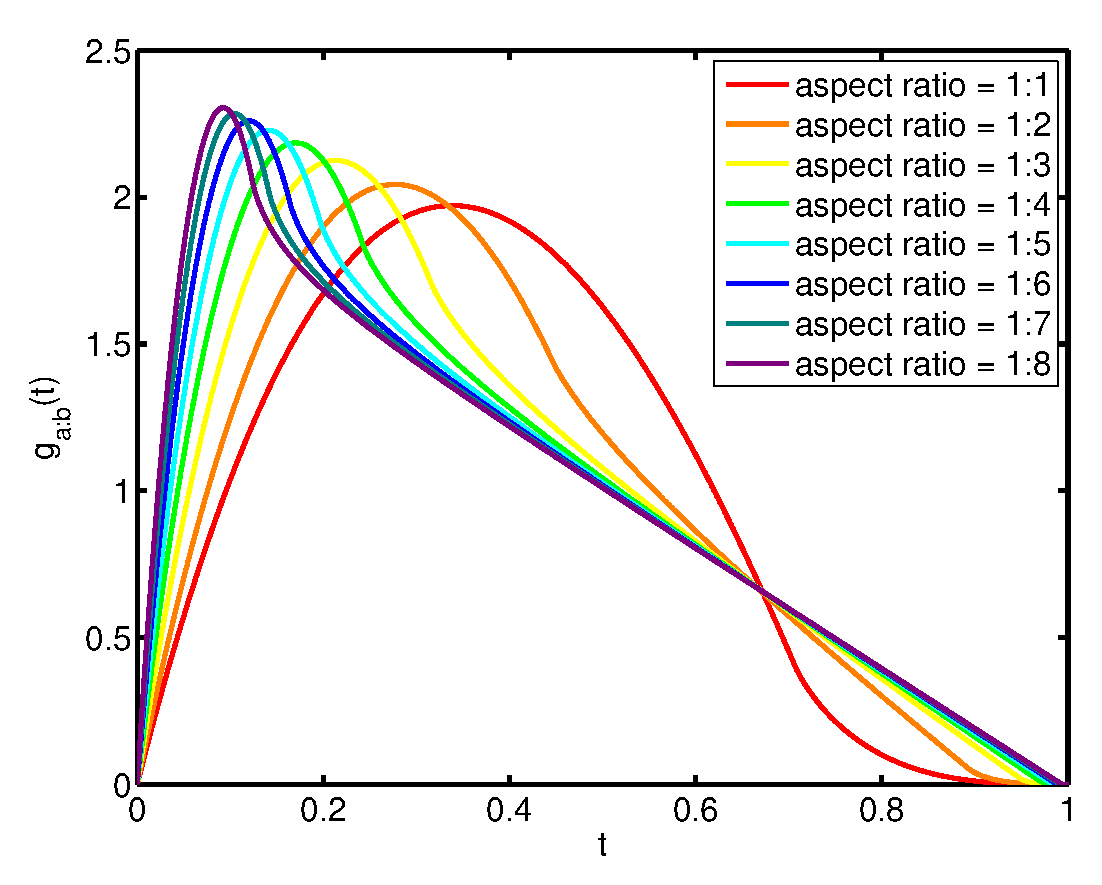
\includegraphics[width=0.33\columnwidth]{Plots/LinePicking_test_rect.eps}}
    \subfloat[\label{fig:b_balls}Density distribution of $n$-D balls.]{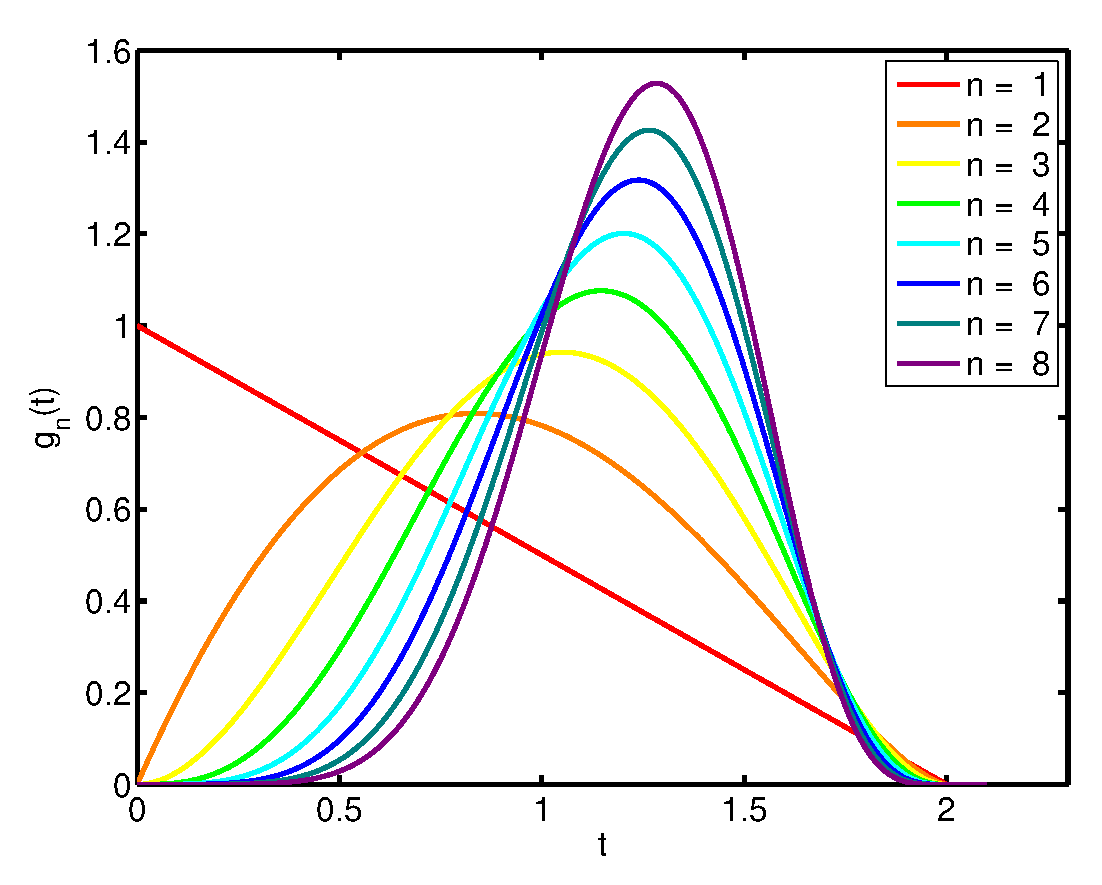
\includegraphics[width=0.33\columnwidth]{Plots/LinePicking_test_balls.eps}}
    \subfloat[\label{fig:various} Various densities distributions for
    shapes with area fixed to 1.]{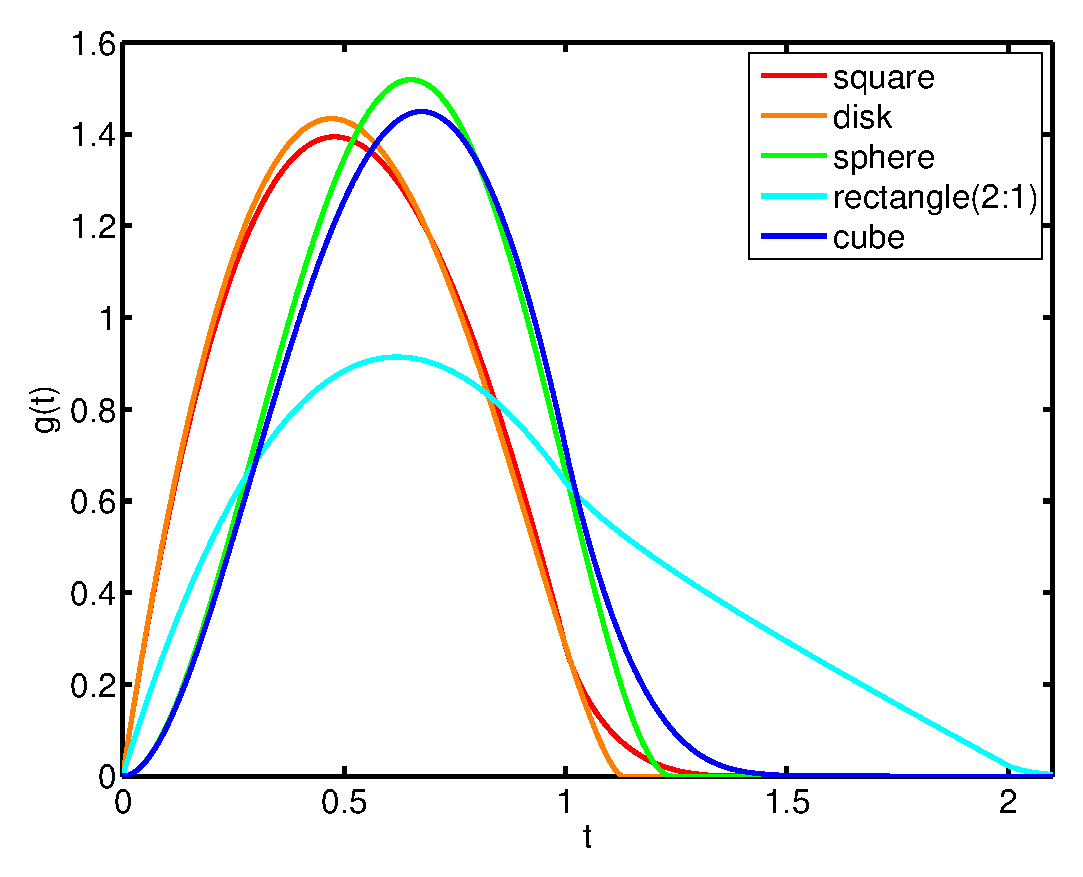
\includegraphics[width=0.33\columnwidth]{Plots/LinePicking_test_fix_area.eps}}
    \caption{Example distance densities.}
  \end{center} 
\vspace{-4mm}
\end{figure}



Note that once again we can derive a small $t$ approximation,
namely, 
\[ g_{a,b}(t) \simeq \frac{4 t}{a^2 b^2} \frac{ab \pi}{2}
            = \frac{2 \pi t}{a b} \]
though here we must assume that the scale-length implied by $\alpha$
is smaller than $a$, the minimum dimension of the rectangle.  Once
again, the approximation is the same as that of the rectangle and
disk, with respect to unit area.




The universality of the small $t$ expansions (used for deriving small
$\alpha$ approximations to the length distributiohn) suggests a
general form
\[ g(t) \simeq \frac{2 \pi t}{A} = 2 \pi d, \]
where $A$ is the area of the region of interest and $d$ is the scaled
distance $d = t/A$. Notice that this scaling is different from the one
used in the Waxman distance function where we scale by the maximum
distnace $L$. 

The above result generalize immediately to Waxman graphs on $n$
dimensional spaces. We simply need to calculate $g(t)$ on the space in
question. For instance, generalizations of $g(t)$ on the
$n$-dimensional ball exist~\cite{tu00:_circle_line}, called the ``ball
line picking'', i.e., for a $n$-dimensional ball of radius $R$,
\[ g_n(t) = n \frac{t^{n-1}}{R^n} I_x\left( 
  \frac{1}{2} (n+1), \frac{1}{2}
                      \right),
\]
where
\[ x = 1 - \frac{t^2}{4 R^2}, \]
and $I_x(p,q)$ is a {\em regularized beta function}
\[  I_x(p,q) = \frac{ B(x; p,q)}{B(p,q)}, \]
where $B(x; p,q)$ is an incomplete beta function, and $B(p,q)$ is a
beta function, i.e., 
\begin{eqnarray*}
  B(p,q)    & = & \int_0^1 t^{p-1} (1 - t)^{q-1} \, dt, \\
  B(x; p,q) & = & \int_0^x t^{p-1} (1 - t)^{q-1} \, dt, \\
\end{eqnarray*}
The first few of these are \cite{tu00:_circle_line} ($P_2$ in (5) and
(17), $P_3$ in (9) and (19), $P_4$ in (18) and $P_5$ in (20), general
even form in (15), general odd form in (16)):
\begin{eqnarray}
  \label{eq:ball_line_picking}
  g_1(t) & = & \frac{1}{R} - \frac{t}{2 R}   \label{eq:line_line_picking} \\
  g_2(t) & = & \frac{4 t}{\pi R^2} \cos^{-1} \left( \frac{t}{2R} \right) 
               - \frac{2 t^2}{\pi R^3} \sqrt{1 - \frac{t^2}{4 R^2} } \label{eq:2dball_line_picking} \\
          & = & \frac{2 t}{R^2} 
               - \frac{2 t^2}{\pi R^3} \sqrt{1 - \frac{t^2}{4 R^2} }
               - \frac{4 t}{\pi R^2} \sin^{-1} \left( \frac{t}{2R} \right) \label{eq:2dball_line_picking2}  \\
  g_3(t) & = & \frac{3 t^2}{R^3} - \frac{9 t^3}{4 R^4} + \frac{3 t^5}{16 R^6}   \label{eq:sphere_line_picking}  \\
  g_4(t) & = &  \frac{8 t^3}{\pi R^4} \cos^{-1} \left( \frac{t}{2R} \right) 
               - \frac{8 t^4}{3 \pi R^5} \left( 1 - \frac{t^2}{4 R^2} \right)^{3/2}
               - \frac{4 t^4}{\pi R^5} \sqrt{1 - \frac{t^2}{4 R^2} } \\
  g_5(t) & = & \frac{5 t^4}{R^5} - \frac{75 t^6}{16 R^6} + \frac{25 t^7}{32 R^8} - \frac{15 t^9}{256 R^{10}}  
  \label{eq:ball_line_picking-end}
\end{eqnarray}
The above cases for which we know the form of the distribution are
straight-forward to compute, but note that the derivation of $g(t)$
just involves a set of integrals that could be numerically
pre-computed for any region of interest.  
 
Figure~\ref{fig:b_balls} shows a comparison of line picking on
balls of various dimensions, and Figure~\ref{fig:various} shows a
comparison of the 2D and 3D balls to the square and cube. We can see
that as long as the areas (volumes) are matched, they appear quite
similar, respectively, though the rectangle varies considerably more.
% plot is similar to http://mathworld.wolfram.com/BallLinePicking.html

It is also numerically straight-forward to compute $g(t)$ where the
points are placed non-uniformly in the region of interest. Some
analytic cases are treated in \cite{tu00:_circle_line}, but for
instance dealing with an inhomogeneous Poisson process used to model
``burstiness'' or clustering of points, and thence with a somewhat
different structure than the standard Waxman graph.


We also know the asymptotic form of these distributions for $t
\rightarrow 0$, i.e., 
\begin{equation}
  \label{eq:asympt_line_picking}
  g_n(t) \simeq n \frac{t^{n-1}}{R^n}
\end{equation}
because we can write % http://en.wikipedia.org/wiki/Beta_function
\begin{eqnarray*} 
   I_x(a,b) 
& = & \sum_{j=a}^{a+b-1} {(a+b-1)! \over j!(a+b-1-j)!} x^j (1-x)^{a+b-1-j} \\
& = & \sum_{j=a}^{a+b-1} {(a+b-1)! \over j!(a+b-1-j)!} 
        \left(1 - \frac{t^2}{4 R^2}\right)^j \left( \frac{t^2}{4 R^2} \right)^{a+b-1-j} \\
& = & \left(1 - \frac{t^2}{4 R^2}\right)^{a+b-1}
       + \sum_{j=a}^{a+b-2} {(a+b-1)! \over j!(a+b-1-j)!} 
        \left(1 - \frac{t^2}{4 R^2}\right)^j \left( \frac{t^2}{4 R^2} \right)^{a+b-1-j} \\
& = & 1 + O(t),
\end{eqnarray*}
and this is directly useful for calculating large $s$ (small $\alpha$)
approximations of the estimator.

For instance, from before, we know that if the $j$th derivative of
$g(t)$ at $t = 0$ is the first non-zero derivative, then the ratio of
Laplace transforms takes the form $\sim (j+1)/s$, so here, it is
immediately obvious that
\[ -G_n(s)/G_n(s) \rightarrow n/s, \]
for large $s$. 

This result is now obvious for the sphere, but for non-spherical (but
convex) regions, we simply need to consider $s$ large enough that the
probability of links longer than $\epsilon$ is negligable, where
$\epsilon$ is chosen so that the chance of intersecting with a
boundary is negligable, and so we can use a spherical
approximation. For instance, the {\em cube line picking} problem has
probability distribution given by \cite{weisstein:_cube_line_picking},
which has first non-zero term of $O(t)$, which is correct for a 2D
space.

We can extend some of this insight into other problems, for instance,
the {\em circle line picking} problem, where pairs of points are
chosen on a circle, but the lines cross the circle. Here, the
probability distribution for line length (with a unit circle) is
\cite{weisstein:_circle_line_picking}
% http://mathworld.wolfram.com/CircleLinePicking.html
\begin{equation}
  \label{eq:circle_line_picking}
  g(t) = \frac{1}{\pi} \left(    
           1 - \frac{s^2}{4}
               \right)^{-1/2} 
       \simeq \frac{1}{\pi} \left( 1 - \frac{s^2}{4} + \cdots \right) 
\end{equation}
whereas in {\em sphere line
  picking}~\cite{weisstein:_sphere_line_picking}, there distribution
takes the form
\begin{equation}
  \label{eq:sphere_line_picking_approx}
  g(t) = \frac{1}{2} t.
\end{equation}
Clearly in this type of case, the dimension of the space is not the
critical factor, because the space on which the points are chosen is
embedded in a larger space from which lines are chosen, and the
geometry of the relationship is important.


INCIDENTALLY -- limit n -> infty for balls, has almost fixed distances
between nodes, so it approaches ER graph


\section{Numerical Computation by Simulation}
\label{sec:numerical}

It may be possible that one wishes to compute distributions, and
resulting Laplace transforms on irregular regions, for which there is
no closed form solution. This can be easily accomplished numerically,
by simulating a cases.

The general process is as follows:
\begin{enumerate}

\item Simulate a set of $2N$ points in the region of interest, and
  calculate the distances between successive pairs. The region may be
  irregular, or even non-convex; decisions may be made about some
  lines being inadmissable (because, for instance, they are exterior
  to the region for a non-convex region), or distances may be
  non-Euclidean, or the point distribution can be non-uniform. All
  that is needed is a set of output distances $\{ t_i \}_{i=1}^{N}$.

\item The density could then be approximate through binning, or a
  kernal smoothing technique, but in fact, we don't need direct access
  to the density as the estimator uses the Laplace transform.

\item We can estimate the Laplace transform as follows:
\begin{equation}
    \label{eq:numerical_laplace}
  \begin{array}{rclcl}
    G(s) & = & \displaystyle \int_0^t g(t) \, dt     & = & \displaystyle \frac{1}{n} \sum_{i=1}^{N} e^{-s t_i}, \\
    G'(s) & = & \displaystyle  \int_0^t t g(t) \, dt & = & \displaystyle \frac{1}{n} \sum_{i=1}^{N} t_i e^{-s t_i}, \\    
  \end{array}
\end{equation}

\end{enumerate}
Note that only one set of points need be generated to estimate the
Laplace transforms for a large set of values of $s$. 

We have tested the above approach, running it 30 times (with different
seeds), in Matlab for various values of $N$. The results are shown in
Figure~\ref{fig:simulated_laplace}. The first plot shows estimates of
the mean relative absolute error of the estimated Laplace transforms
over the range $S \in [0, 50]$. We can see from the fitted straight
line, that the errors decrease as $1/\sqrt{N}$, dropping to around 1\%
at around $N=100,000$.

The second plot shows the computation times\footnote{Both algorithms
  were implemented in Matlab, the exact method using Matlab's {\tt
    quadqk} function. } relative to the computation times for the
``exact'' method\footnote{Note that both techniques are in some
  respect numerical, because even when we have a closed form solution
  for the density, we still typically need to numerically integrate
  this to obtain the Laplace transform, but we shall refer to this
  solution as ``exact'' for the sake of clarity in the following
  results, and because in the following we perform numerical
  integration with error tolerances of $10^{-6}$, which means the
  errors in this approach are significantly smaller than those of the
  simulation-based approach, at least for the ranges of $N$ tested
  here.}  We can immediately notice that computation times are roughly
linear in $N$, as one might expect. that around the range $N=100,000$,
the simulation approach is competitive with the exact approach.

The simulation-based approach is not as accurate as the exact
numerical approach, however, it accuracy should be sufficient for most
estimation problems, without increasing the computational workload
unduly.

\begin{figure}[tbp]
  \begin{center}
    \subfloat[Mean relative error in $-G'(\hat{s})/G(\hat{s})$.]{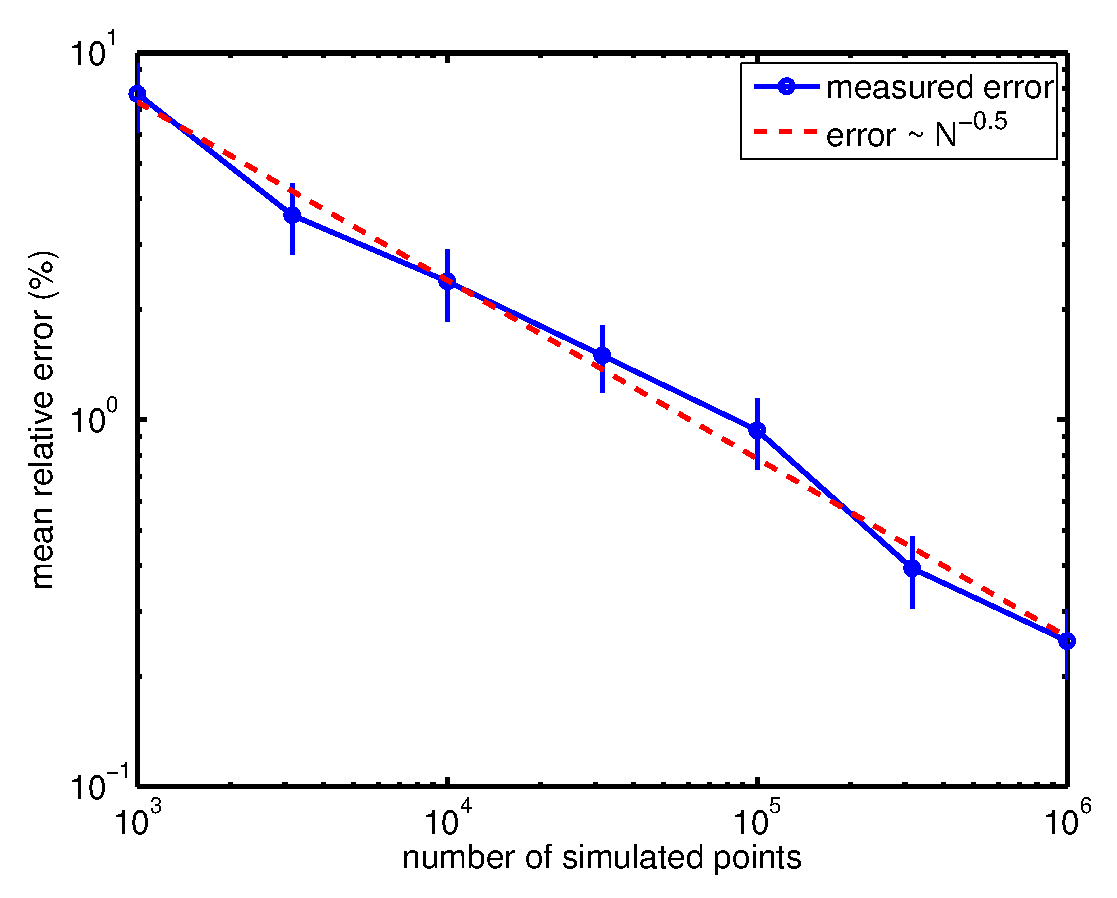
\includegraphics[width=0.49\columnwidth]{Plots/LinePicking_numerical_rel_error.eps}}
    \subfloat[Relative computation time of the simulation-based
    approach, with respect to the exact approach.]{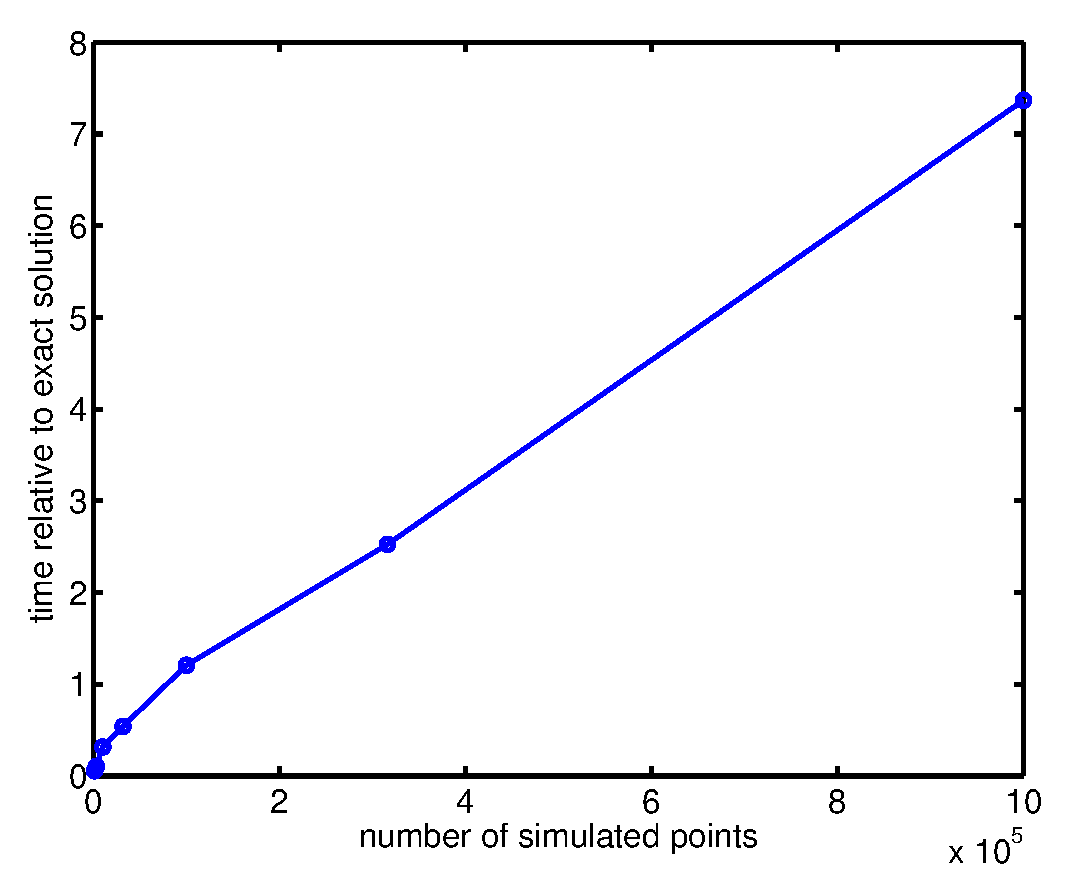
\includegraphics[width=0.49\columnwidth]{Plots/LinePicking_numerical_time.eps}}
    \caption{A comparison of simulation-based Laplace transform
      calculation with the exact approach.\label{fig:simulated_laplace}}
  \end{center} 
\vspace{-4mm}
\end{figure}

We could further use the above in the estimator as follows: we aim to
find the value $\hat{s}$ such that $-G'(\hat{s})/G(\hat{s}) = \bar{d}$,
so 
\begin{eqnarray*}
  -G'(\hat{s}) & = & \bar{d} G(\hat{s}) \\
  \frac{1}{n} \sum_{i=1}^{N} t_i e^{-s t_i}    & = & \bar{d} \frac{1}{n} \sum_{i=1}^{N} e^{-s t_i} \\
  \sum_{i=1}^{N} (t_i - \bar{d} ) e^{-s t_i}  & = & 0
\end{eqnarray*}
We could feed this new function directly into our search algorithm to
find the estimate, avoiding the need to calculate both $-G'(\hat{s})$
and $G(\hat{s})$ for multiple values of $s$. This approach has other
advantages as well:
\begin{itemize}

\item The gradient of this function is immediately obvious, and not
  problem specific as it is for closed form solutions, leading to
  generic estimation functions;

\item We could approach the estimation iterative, for intance, by
  generating $M$ point, performing an estimate, and then refining it
  with the next $M$ points, continuing until the results converge on a
  solution with some desired tolerance.

\end{itemize}



\section{Programs}
\label{sec:program}

\subsection{A Rough Guide}

\subsection{Numerical Issues}


\section{Correlations}

Correlations between distances \cite{bartlett64}

(0) correlation between a pair 1/10

(i) $n$ nodes, then $N = n (n-1)/2$ pairs of nodes, and so this many pairs of distances

(ii) the $N (N-1) /2 = n (n-1) (n (n-1) -1)/8 = $ possible pairs of
correlations

(iii) but only $n(n-1)(n-2)/2$ of the correlations are positive,
because they share a node so we get average correlation between all
pairs
 \[ \frac{1}{10} \frac{n(n-1)(n-2)/2}{n (n-1) (n (n-1) -1)/8} =
    \frac{2}{5} \frac{(n-2)}{(n (n-1) -1)}
   \simeq 
   \frac{2}{5n}
\]
for large $n$

Empirical measurement (see triples.m)
\[ r = 0.114865 \pm 0.000037\]


\section{Conclusion and Future Work}




\setlength{\parskip}{1mm}
\bibliographystyle{ieeetr}
\bibliography{queueing_theory,books,ip_traffic,time_series,reliability,tcp,ospf,lrd,worms,internet,routing,bgp,topology,network,traffic_engineering,algorithms,optimization,history,graph}

\end{document}


